\documentclass[11pt,a4paper]{ivoa}
\input tthdefs

\usepackage{appendix}
\usepackage{listings}
%\lstloadlanguages{sh,make,xml,[latex]tex}
\lstset{flexiblecolumns=true,numberstyle=\small,showstringspaces=False,
  identifierstyle=\texttt,defaultdialect=[latex]tex,language=tex}


\title{IVOA Interoperable Authentication Process \\ for non browser clients}

\ivoagroup{http://www.ivoa.net/twiki/bin/view/IVOA/IvoaGridAndWebServices}

%\author[????URL????]{http://www.ivoa.net/twiki/bin/view/IVOA/IvoaGridAndWebServices}
%\textcolor{red}{Editor's note: Author list to be completed}
\author{Patrick Dowler}
\author{Mark Taylor}
\author{Sara Bertocco}

\editor{Sara Bertocco}

%\previousversion[http://www.ivoa.net/documents/SSO/20160930/index.html]{WD-20160930}



\begin{document}

\begin{abstract}
IVOA's Interoperable Authentication Management explains how 
IVOA non-browser clients and services can manage the 
authentication process 
to be interoperable. Particularly, this document
describes how services advertise their
support of specific authentication schemes and how
clients can discover and use these information to access protected 
resources.

\end{abstract}

\section*{Acknowledgments}
\textcolor{red}{Editor's note: this section has to be 
updated/rewritten. Authors who have someone to thank should
add here acknowledgments}
This document derives from discussions among the Grid and Web Services
working-group of IVOA. It is particularly informed by prototypes built
by Mark Taylor (University of Bristol) and Patrick Dowler
(Canadian Astronomy Data Centre).



\section*{Conformance-related definitions}
The words ``MUST'', ``SHALL'', ``SHOULD'', ``MAY'', ``RECOMMENDED'', and
``OPTIONAL'' (in upper or lower case) used in this document are to be
interpreted as described in IETF standard, \citet{std:RFC2119}.

The \emph{Virtual Observatory (VO)} is
general term for a collection of federated resources that can be used
to conduct astronomical research, education, and outreach.
The \href{http://www.ivoa.net}{International
Virtual Observatory Alliance (IVOA)} is a global
collaboration of separately funded projects to develop standards and
infrastructure that enables VO applications.


\section{Introduction}
This document considers the authentication process in a VO context
where services belonging to different realms
\textcolor{red}{to be checked}
interoperate. The use 
case we are going to face is:\\
a user client contacts a service (providing resources) and needs: \begin{itemize}
    \item to know if authentication is required
    \item if yes, a URL for login endpoint(s),
    \item the API of the login endpoint(s),
    \item the kind of credential the endpoint(s) will return
\end{itemize}
While this use case is already solved in web applications,
where it is the browser mediation and authentication schemas 
are standardized (see
IETF\footnote{https://www.ietf.org/}), it is open
in case of non-browser clients and for what concerns the
interoperability.


\subsection{Role within the VO Architecture}

\begin{figure}
\centering

% Get the architecture diagram from the TCG chair
% http://wiki.ivoa.net/twiki/bin/view/IVOA/IvoaTCG
% If they give you a PDF, for now dumb it down to a png by
% convert -antialias -density 72x72 archdiag.pdf archdiag.png
% Oh -- Notes don't need this; you'd have to remove archdiag.png
% from FIGURES in the Makefile, too.
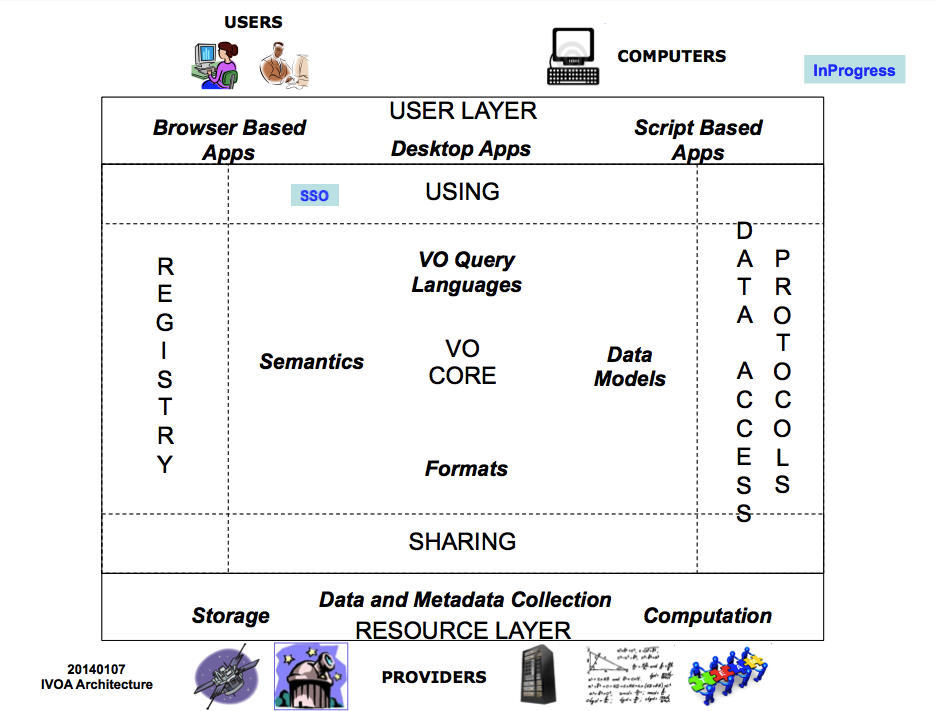
\includegraphics[width=0.9\textwidth]{IVOA-IAM_image001.png}
\caption{Architecture diagram for this document}
\label{fig:archdiag}
\end{figure}

Fig.~\ref{fig:archdiag} shows the role this document plays within the
IVOA architecture \citep{2010ivoa.rept.1123A}.

\section{Glossary}
\begin{itemize}
  \item[{\bf challenge}] is an RFC 7235 WWW-Authenticate HTTP 
  response header indicating accepted authentication options
  \item[{\bf supported challenge}] is a challenge that the AUTH 
  library understands (currently \texttt{ivoa\_cookie}, 
  \texttt{ivoa\_x509}, basic)
  \item[{\bf domain}] is a set of resources with the same 
  authentication arrangements; membership rules are challenge-type 
  specific
\end{itemize}


\section{The authentication process}

In the IVOA authentication process, the authentication is conveyed
using {\emph WWW-Authenticate} challenges as defined by
IETF RFC 7235 \citep{rfc7235}.\\
The basic form of the header in an authentication challenge is:

\begin{verbatim}
www-authenticate: {auth-scheme} {scheme-specific-params}
\end{verbatim}
Where \emph{auth-scheme} is a reference to the authentication 
schema,
and \emph{scheme-specific-params} conveys the authentication
service-specific details, i.e. the authentication end-point
and how to manage the authentication.\\
Any endpoint can return a www-authenticate challenge  
in any response, particularly both to a 
``first call'' and when something changes (for example, a token
expires or an attempt to access a protected resource is made).\\
Multiple challenges may be in a service's
response. Clients can choose whichever one they understand or prefer.

\subsection{Bootstrapping}
"How to know if authentication is required? 
How does a client start and how does a service signal 
that there is
\emph{optional}, \emph{required}, or \emph{no} authentication?"

Clients initially find the level of authentication
(bootstrap), making anonymous HTTP GET or HTTP HEAD requests to
the service's /capabilities endpoint. (See VO Support Interfaces (VOSI)
(\citep{2017ivoa.spec.0524G}.)
\textcolor{red}{Editor's note: How can the client know the
endpoint of the capability service? Someone told parsing the
contacted service endpoint, but what are the parsing rules?}
Generic form of the responses from this call to /capabilities is:
\begin{verbatim}
HTTP/1.1 200 OK
Server: DaCHS/2.10 twistedWeb/22.4.0
Date: Thu, 07 Nov 2024 15:27:07 GMT
WWW-Authenticate: Basic realm="Gavo"
Content-Type: text/xml
\end{verbatim}
The HTTP status codes in the response header can be:
\begin{itemize}
\item [{\bf HTTP status code {\emph{200}}}] with no www-authenticate headers (supported challenge) 
default to {\bf{\emph{no authentication}}}. If www-authenticate headers (supported challenge) 
is specified, then optional authentication can be performed.
\item [{\bf HTTP status code {\emph{401}}}] with 
www-authenticate headers: {\bf{\emph unauthorized}}. This case happen
when an access token is missing or is expired, revoked, malformed,
or invalid for other reasons. So authentication is required.
The service response MUST include in the WWW-Authenticate header the authentication scheme to use and a login end-point.
\item [{\bf HTTP status code {\emph{403}}}] with www-authenticate
headers: {\bf{\emph forbidden}}. 
With this status code, the API tells the client that the credentials it 
provided (e.g., an access token) are valid, but it needs 
appropriate privileges to perform the requested action.
The service response must include in the WWW-Authenticate header the authentication 
scheme to use and a login end-point.
\textcolor{red}{[Editor's note: The API 
may include what privileges are needed in its response. But
a description is needed and this open the problem to define 
scopes and how to use them (also among different realms).
NEEDS REVIEW}
\end{itemize}

\textcolor{red}{[Note: two changes to VOSI are required: 1) VOSI augmented to
require http HEAD support for /capabilities endpoints, and 2) Modify
VOSI to allow /capabilities to respond with 401 (or 403) (also affects
TAP 1.1 sec 2; \&\ others?)]}


\subsection{Authentication Discovery}
As already described, services SHOULD
advertise that they support authentication through the use of
\emph{WWW-Authenticate} HTTP response headers, as defined by
IETF RFC 7235 \citep{std:RFC7235}. 

The service that provides authentication should advertise clients, 
in the response, whether or not they successfully authenticated using:
\begin{verbatim}
X-VO-Authenticated: true|false
\end{verbatim}
that can be both in the response HEADER and in the response BODY. 
Services may choose to include the X-VO-Authenticated header in all
requests (not just to /capabilities) made where user authentication was successful.

In the authentication process, the service must identify the user 
and return the username or the X.509 distinguished name.


\section{Supported challenges}
The set of supported challenges, {\bf ivoa\_cookie},
{\bf ivoa\_x509} and login-password ({\bf basic}) authentication
rely on existing prototypes.

\subsection{ivoa\_cookie}
The authentication with cookies refers to the IETF RFC 2965 \citep{rfc6265}, with additional parameters indicating where/how to get a cookie.\\
A service that support authentication through cookie SHOULD
respond to a call to its capability service with an header
of the form
\begin{verbatim}
www-authenticate: ivoa_cookie 
           standard_id="ivo://ivoa.net/sso#tls-with-password", 
           access_url="https://example.org/login"
\end{verbatim}
As seen above, the \emph{auth-scheme} points authentication 
through cookies, while the \emph{scheme-specific-params} contains 
two standard parameters:
\begin{itemize}
\item{\emph{standard\_id}} - describes how to obtain the 
credentials i.e. cookies can be obtained exchanging
username and password with TLS encryption;
\item{\emph{access\_url}} - describes where to go to type
username and password and obtain the credentials (cookie)
\end{itemize}


\subsubsection{Example}
The following is an example of a working prototype.
\begin{verbatim}
% curl -sI https://geadev.esac.esa.int/tap-server/tap/capabilities \
| grep ivoa_cookie
WWW-Authenticate: ivoa_cookie \
     standard _id="ivo://ivoa.net/sso#tls-with-password", \
     access url="https://geadev.esac.esa.int/tap-server/login"
\end{verbatim}


\subsection{ivoa\_x509}
The authentication with X.509 certificates, requires additional parameters 
indicating where/how to get one certificate. \\
A service that supports authentication through X509 certificates SHOULD
respond to a call to its capability service with a header
of the form
\begin{verbatim}
www-authenticate: ivoa_X509 
           standard_id="ivo://ivoa.net/sso#tls-with-password", 
           access_url="https://example.org/login"
\end{verbatim}

The \emph{auth-scheme} points authentication 
through X509 certificates (including self-signed
proxy certificates), while the \emph{scheme-specific-params} contains  
two standard parameters. There are two variants: one with the two
parameters, \emph{standard\_id}, and \emph{access\_url}, and one without. The
one with parameters tells the clients they can get an acceptable client
certificate via the described mechanism. (For sites that provide their own cert
certificate authority.) 
\begin{itemize}
\item{\emph{standard\_id}} - describes how to obtain the 
credentials i.e. X509 certificate can be obtained exchanging
username and password with TLS encryption;
\item{\emph{access\_url}} - describes where to go to type
username and password and obtain the credentials (X509 certificate)
\end{itemize}
The second one, without params, says that the
service accepts client certificates from an external certificate
authorities.
\textcolor{red}{Editor's note: need to clarify the case without 
parameters: if the user is not authenticated, how to know where 
to go to get a certificate?}

\subsubsection{Example}
The following is an example of a working prototype.
\begin{verbatim}
% curl -sI https://ws.cadc-ccda.hia-iha.nrc-cnrc.gc.ca/argus/capabilities \
| grep ivoa x509
www-authenticate: ivoa_x509 \
   standard_id="ivo://ivoa.net/sso#BasicAA", \ 
   access url="https://ws.cadc-ccda.hia-iha.nrc-cnrc.gc.ca/cred/auth/priv" \
www-authenticate: ivoa_x509
\end{verbatim}

\subsection{Basic}
This is simply HTTP Basic authentication as described by 
the IETF RFC 7617 \citep{rfc7617}, no VO customisation is 
required. A service that supports basic authentication, 
through a login-password form, SHOULD respond to a call 
to its capability service with a header of the form
\begin{verbatim}
WWW-Authenticate: Basic realm="realm_name"
\end{verbatim}
The \emph{auth-scheme} points authentication Basic and
no \emph{scheme-specific-params} are required.
\textcolor{red}{Where is the link of the form where the user inputs login and password?}


\subsubsection{Example}
The following is an example of a working prototype.
\begin{verbatim}
% curl -sI http://dc.g-vo.org/tap/capabilities | grep Basic
WWW-Authenticate: Basic realm="Gavo"
\end{verbatim}

\section{The OAuth2 case}

\subsection{Glossary}
\begin{itemize}
\item[{\bf OAuth 2 Authorization Server}](from RFC 6749 \citep{rfc6749}): 
    is the server 
    issuing access tokens to the client after successfully authenticating 
    the resource owner and obtaining authorization.
\item[{\bf OAuth 2 Resource Server}](from RFC 6749 \citep{rfc6749}):
    is the server hosting the
    protected resources, capable of accepting and responding to
    protected resource requests using access tokens.\\
    In the VO context, this would be a TAP/SCS/etc. service.
\item[{\bf OAuth 2 Client}]: is an application making protected
    resource requests on behalf of the resource owner and with its
    authorization.\\
    In the VO contact, this would be Aladin, pyvo, TOPCAT and
    similar clients (as would be expected).
\item[{\bf VO Discovery Service}]: \\
    A new service which aims to be a minimal
    bridge between OAuth 2.x/OIDC Authorization servers and VO Clients
    that are not browser-based.
\end{itemize}

\subsection{Authentication process steps}
This section covers the case of authentication through the
OAuth2 authorization framework \citep{rfc6749}. 
The use of existing standard flows/grants 
is recommended fostering the use of off-the-shelf 
OAuth 2.x/OIDC authentication providers.
Minimal changes to the existing standards are needed for
non-browser clients. Non-browser clients should not be required
to call out a browser, nor run a web server for redirects (this
covers situations where clients are running on a remote server 
or are otherwise unable to contact a browser directly)

Steps to obtain authentication:
\begin{enumerate}
    \item In order for an OAuth 2.0 [RFC6749] client to utilize an OAuth 2.0
   authorization server, the client needs specific information to
   interact with the server, including an OAuth 2.0 client identifier to
   use at that server.  This specification describes how an OAuth 2.0
   client can be dynamically registered with an authorization server to
   obtain this information.
   \item ciao
\end{enumerate}




%\appendix
%\section{standard\_id's}
\appendixtitleon
\appendixtitletocon
\begin{appendices}
\section{standard\_id's}
IVOA standard identifiers for authentication types are in the table.
\begin{table}[th]
\begin{tabular}{p{0.45\textwidth}p{0.64\textwidth}} \sptablerule
\textbf{Authentication type}&\textbf{\xmlel{standard\_id}}\\ \sptablerule
 HTTP Basic Authentication &
\xmlel{ivo://ivoa.net/sso\#BasicAA}\\
TLS with password &  \xmlel{ivo://ivoa.net/sso\#tls-with-password} \\
TLS with client certificate & \xmlel{ivo://ivoa.net/sso\#tls-with-certificate} \\
Cookies & \xmlel{ivo://ivoa.net/sso\#cookie} \\
Open Authentication & \xmlel{ivo://ivoa.net/sso\#OAuth} \\
SAML &  \xmlel{ivo://ivoa.net/sso\#saml2.0} \\
OpenID &  \xmlel{ivo://ivoa.net/sso\#OpenID} \\
\sptablerule
\label{table:SMtable}
\end{tabular}
\end{table}

\section{Useful documents}
The IVOA refers to already existing standards as far as possible and 
integrates them where necessary to achieve interoperability of virtual 
observatory services. This appendix lists already existing standard
documents providing the ecosystem underlying this document.

{\bf RFC 6749 \citep{rfc6749}}:\\ 
    The OAuth 2.0 standard. Note that usage of `Bearer` is covered in
    [RFC 6750]\citep{rfc6750}. There are numerous
    extensions/additions/modifications on top of this. OAuth 2.1 is still in
    draft form, but merges in most of these extensions.

{\bf OpenID Connect Core 1.0: \\
    (\texttt{https://openid.net/specs/openid\--connect\--core\--1\_0.html})}:\\
    This is an extension of RFC 6749 which adds profile/identity related
    information. Usually this is abbreviated as \emph{OIDC} (for Open ID
    Connect).

{\bf OpenID Connect Discovery 1.0}:\\
    It is described how to find out what the endpoints are of an OIDC provider.

{\bf OpenID Connect Dynamic Client Registration 1.0: \\
    (\texttt{https://openid.net/specs/openid\--connect\--registration\--1\_0.html})}:\\
    How to acquire a ``client\_id'' and ``client\_secret'' is described.

{\bf RFC 8628\citep{rfc8628}}:\\ 
    The Device  Authorization Grant.

{\bf RFC 8414\citep{rfc8414}}:\\ 
    Authorization Server Metadata. OAuth 2.x version of OpenID Connect Discovery, and aims to be compatible with it.

{\bf RFC 7591 \citep{rfc7591}}:\\ 
    OAuth 2.x version of OpenID Connect Dynamic Client 
    Registration. There is a companion RFC 7592\citep{rfc7592}.

{\bf RFC 8252 \citep{rfc8252}}:\\
    OAuth 2.0 for Native Apps.
    

\end{appendices}

\bibliography{ivoatex/ivoabib,ivoatex/docrepo,IVOA-IAM}


\end{document}
